\section{Vector-Valued Functions}
\subsection{Vector Fields}
\begin{defn}[Vector Field]
	\sloppy A \textbf{vector field} in $\R^n$ is a map
	\[\mathbf{V}: U \subseteq \R^n \rightarrow \R^n\]
	that assigns each $x$ in its domain $U$ a vector $\mathbf{V}(x)$. 
\end{defn}

\begin{marginfigure}
	A map $\mathbf{V}: U \subseteq \R^n \rightarrow \R$ assigning a number to each point is a \textbf{scalar field}. 
\end{marginfigure}

\begin{marginfigure}
	A vector field on $\R^n$ has $n$ components. If each component is a $C^k$ function, then the vector field is said to be of class $C^k$.
\end{marginfigure}

\begin{ex}{Describing Rotary Motion using a Vector Field}{label}
	Rotary motion can be described by the vector field,
	\[\mathbf{V}(x, y) = -y \mathbf{i} + x \mathbf{j}\]
	\begin{center}
    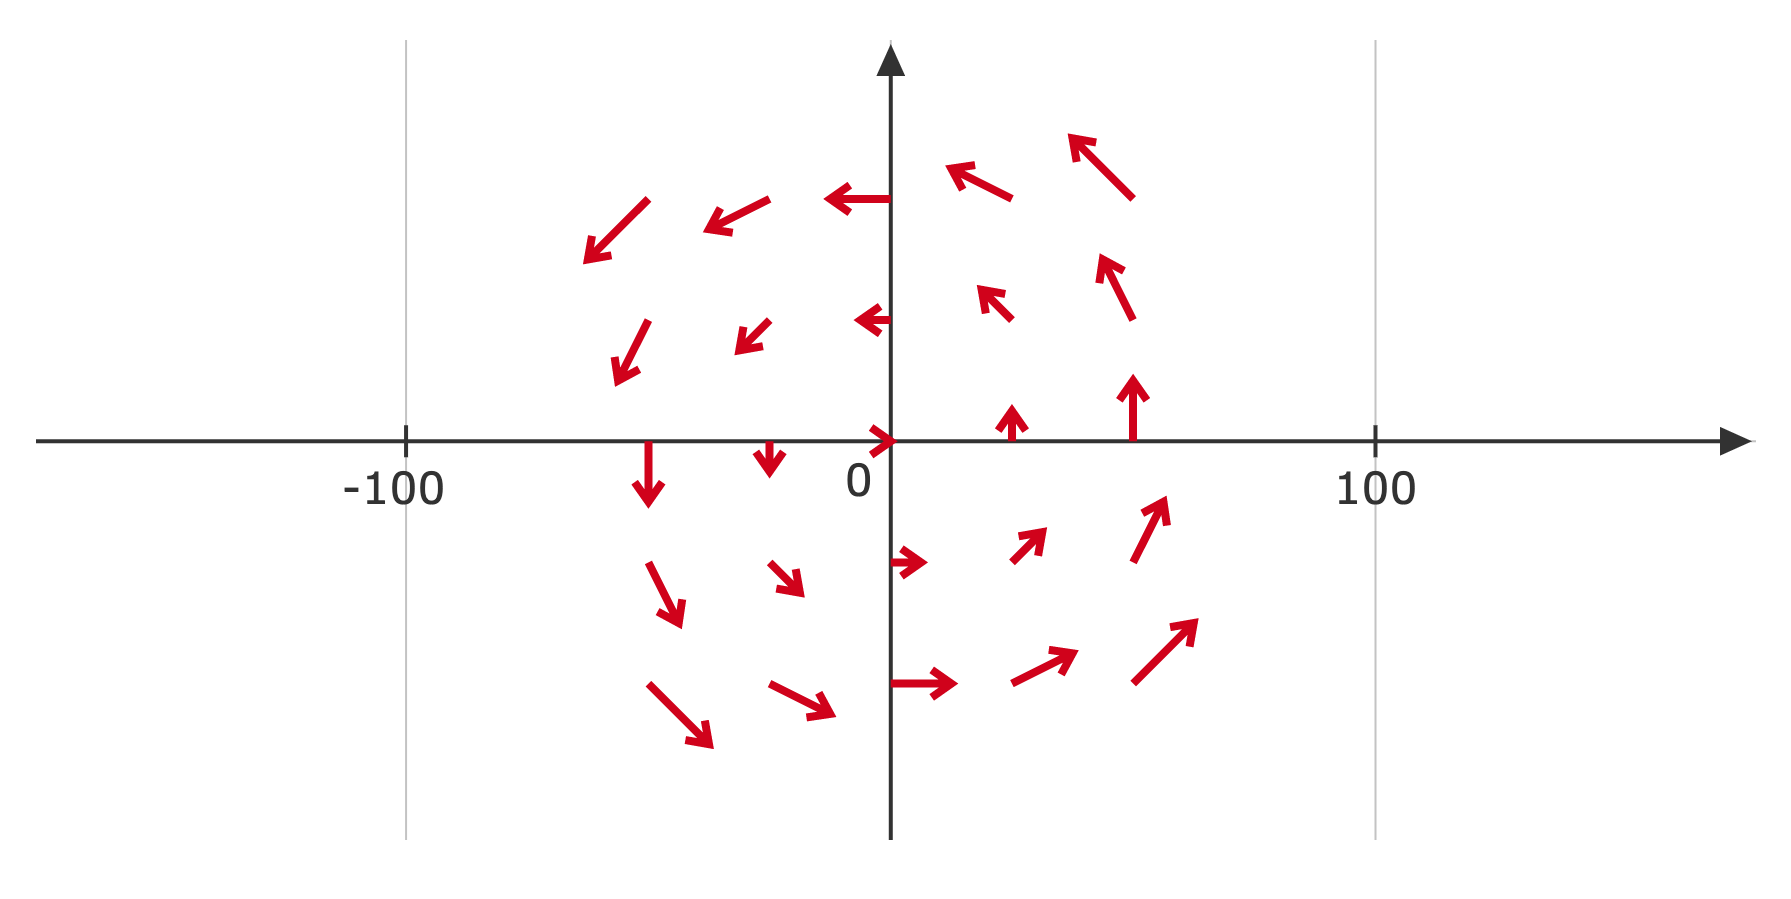
\includegraphics[width=0.7\linewidth]{figures/wk-6/fig-1.png}
	\end{center}
\end{ex}

\begin{ex}{Unit Length Vector Fields}{label}
	The vector field $\mathbf{V}$ defined by,
	\[\mathbf{V}(x, y)=\frac{x}{\sqrt{x^2+y^2}} \cdot \mathbf{i}+\frac{-y}{\sqrt{x^2+y^2}}  \cdot \mathbf{j}\]
	has unit length. It is not defined at the origin,
	\begin{center}
    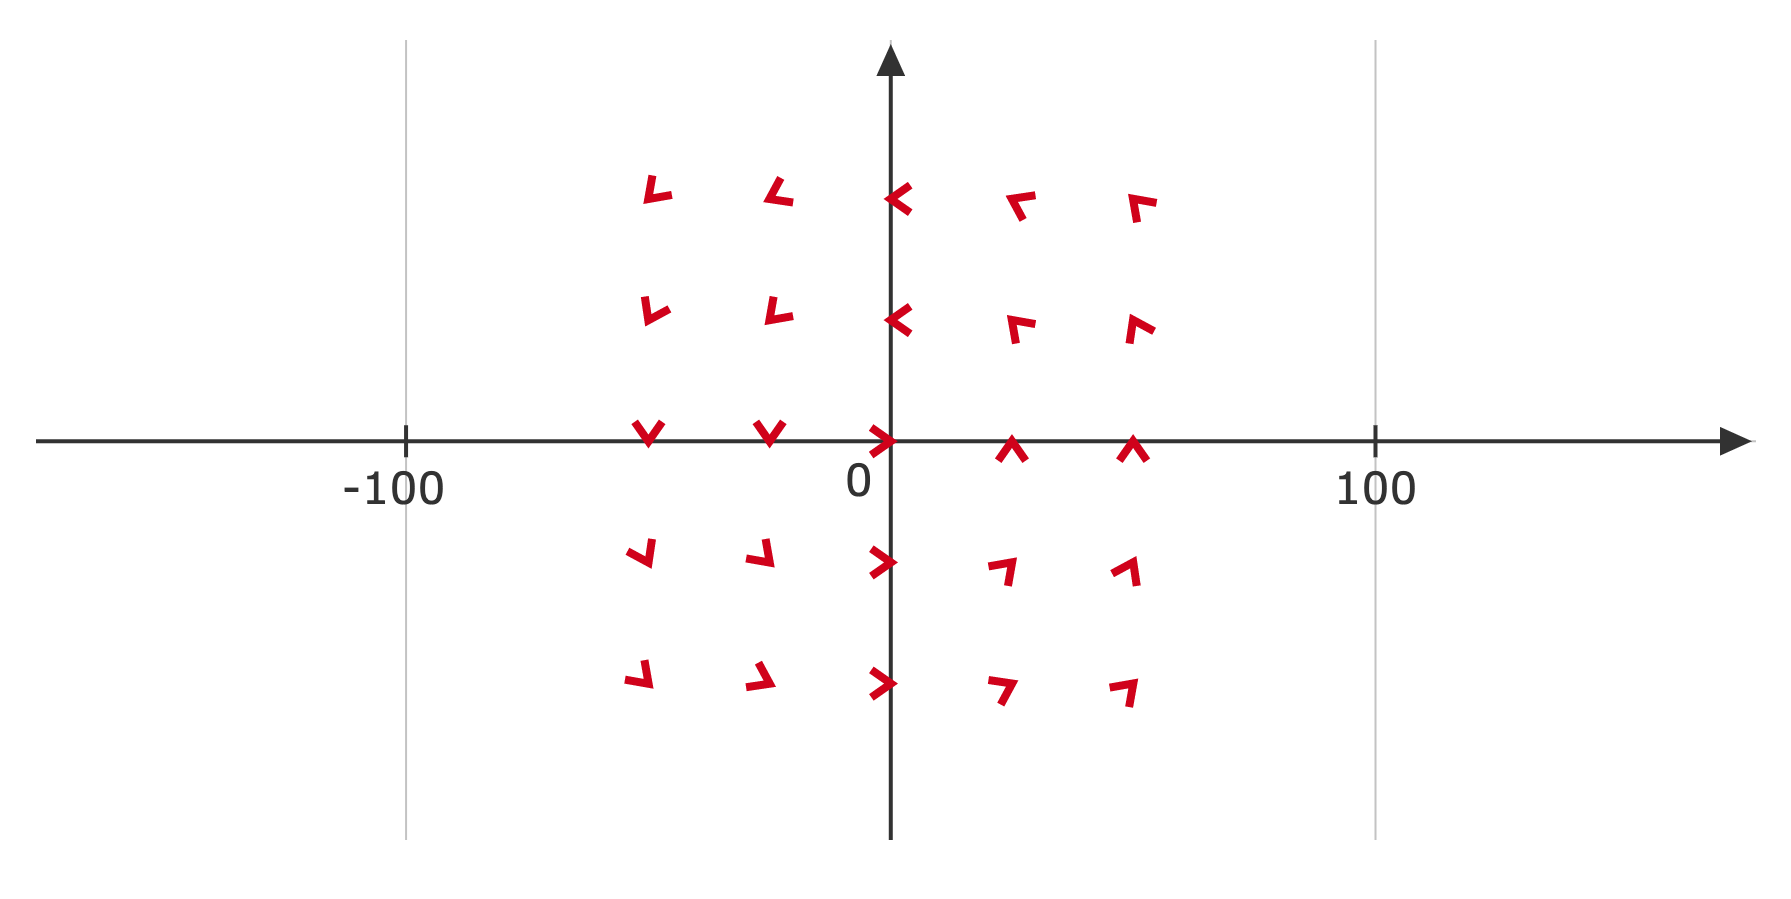
\includegraphics[width=0.7\linewidth]{figures/wk-6/fig-2.png}
	\end{center}
\end{ex}

\begin{ex}{Gradient Vector Fields}{label}
	The gradient of a $C^1$ function is given by,
	\[\nabla f(x, y, z)=\frac{\partial f}{\partial x}(x, y, z) \cdot \mathbf{i}+\frac{\partial f}{\partial y}(x, y, z) \cdot \mathbf{j}+\frac{\partial f}{\partial z}(x, y, z) \cdot  \mathbf{k}\]
	We can think of this as an example of a vector field $\mathbf{V}$.
\end{ex}

\begin{ex}{Identifying Gradient Vector Fields}{label}
	\begin{itemize}
		\item $\mathbf{V}(x, y) = -y \mathbf{i} + x \mathbf{j} $ is not a gradient vector field because the mixed partials $\mathbf{V}_{xy}$ and $\mathbf{V}_{yx}$ are not equal,
		\[\mathbf{V}_x = -y \quad \text{ and } \quad \mathbf{V}_y = x\]
		\item $\mathbf{V}(x, y) = y \mathbf{i} + x \mathbf{j} $ is a conservative because the mixed partials $\mathbf{V}_{xy}$ and $\mathbf{V}_{yx}$ are equal to $1$,
		\[\mathbf{V}_x = y \quad \text{ and } \quad \mathbf{V}_y = x\]
	\end{itemize}
\end{ex}

\begin{ex}{Equipotential Surfaces}{label}
	Given the gradient of $V$,
	\[\nabla V = (x, 2y, 3z) = x \mathbf{i} + 2 \mathbf{j} + 3 \mathbf{z}\]
	we can recover the original function $V: \R^2 \rightarrow \R$,
	\[V = \frac{1}{2}x^2 + y^2 + \frac{3}{2}z^2\]
	The level curves of $V$ are called \textbf{equipotential surfaces}.
\end{ex}

\begin{marginfigure}
	\begin{center}
	    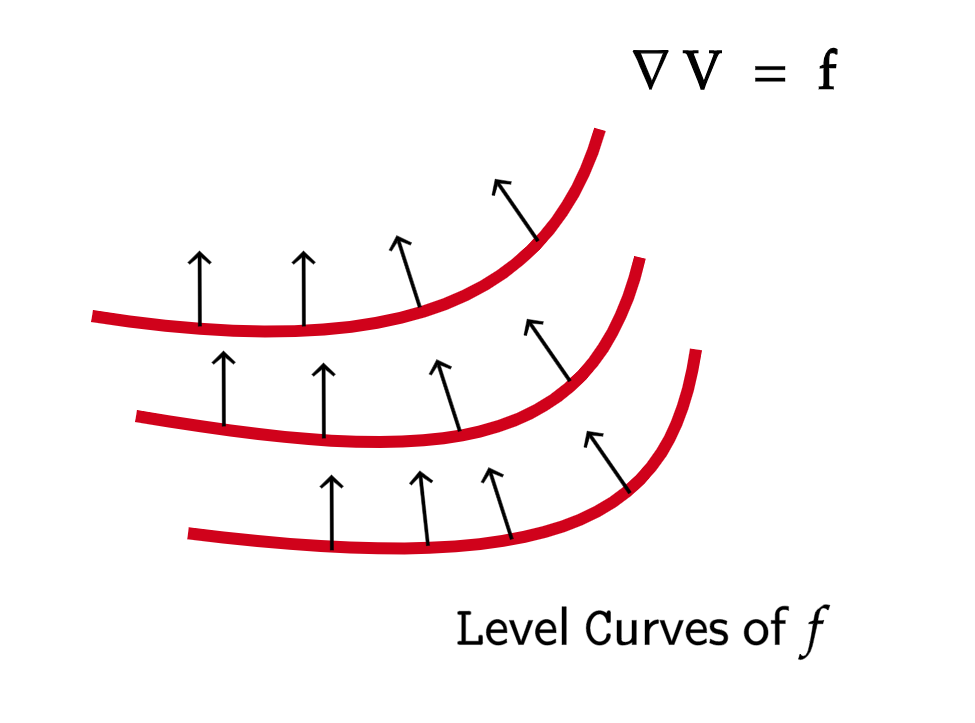
\includegraphics[width=0.7\linewidth]{figures/wk-5/fig-1.png}
	\end{center}
\end{marginfigure}

\begin{defn}[Flow Line]
	A \textbf{flow line} $\mathbf{c}(t)$ for a vector field $\mathbf{V}$ has
	\[\mathbf{c}'(t) = \mathbf{V}(\mathbf{c}(t))\]
\end{defn}

\begin{ex}{Rays}{label}
	Consider the vector field $\mathbf{V}(x, y) = x \mathbf{i} + y \mathbf{j}$, where $\|\mathbf{V}\| = r$.
	\[\underbrace{x^{\prime}(t) \cdot \mathbf{i}+y^{\prime}(t) \cdot \mathbf{j}}_{\mathbf{c}^{\prime}(t)}=\underbrace{x(t) \cdot \mathbf{i}+y(t) \cdot \mathbf{j}}_{\mathbf{F}(\mathbf{c}(t))}\]
	gives the following differential equation,
	\begin{align*}
	&x^{\prime}(t)=x(t) \implies x(t) = c_1 \cdot e^t\\
	&y^{\prime}(t)=y(t) \implies y(t) = c_2 \cdot e^t
	\end{align*}
	implying that the flow lines are rays through the origin.
	\begin{center}
	    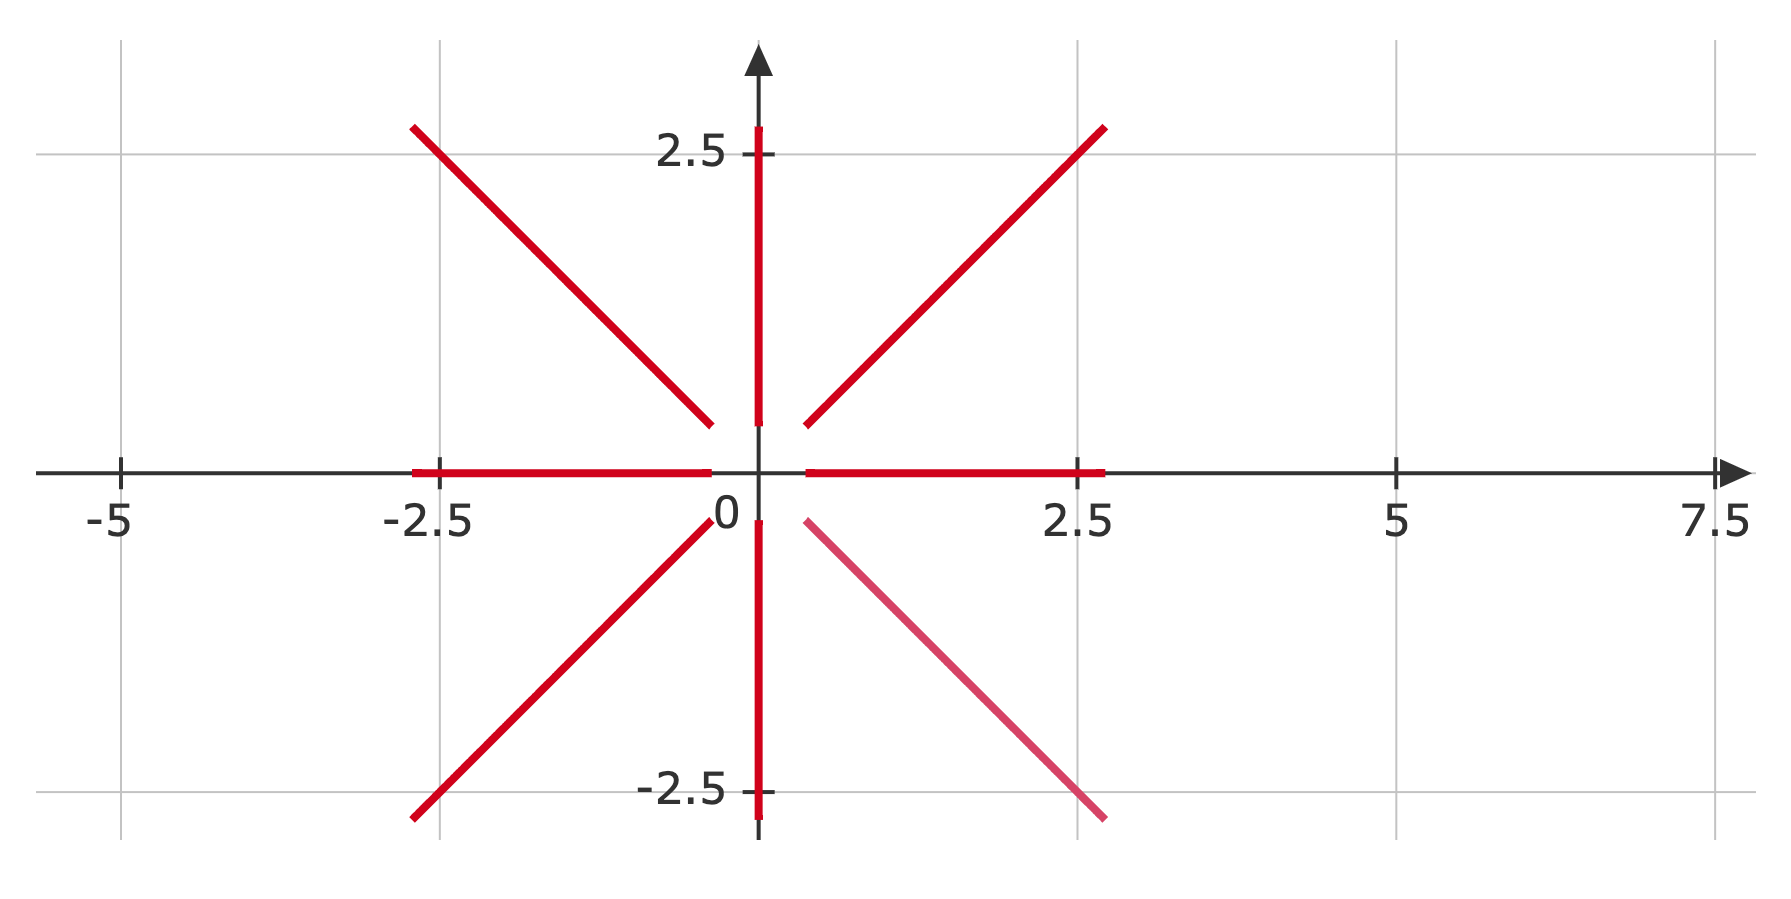
\includegraphics[width=0.7\linewidth]{figures/wk-6/fig-4.png}
	\end{center}
\end{ex}

\begin{ex}{Concentric Circles}{label}
	Consider the vector field $\mathbf{V}(x, y) = x \mathbf{i} - y \mathbf{j}$, where $\|\mathbf{V}\| = r$.
	\[\underbrace{x^{\prime}(t) \cdot \mathbf{i}-y^{\prime}(t) \cdot \mathbf{j}}_{c^{\prime}(t)}=\underbrace{x(t) \cdot \mathbf{i}+y(t) \cdot \mathbf{j}}_{\mathbf{F}(\mathbf{c}(t))}\]
	gives the following differential equation,
	\begin{align*}
	&x^{\prime}(t)=x(t) \implies x(t) = c_1 \cdot \cos t\\
	&y^{\prime}(t)=y(t) \implies y(t) = c_2 \cdot \sin t
	\end{align*}
	implying that the flow lines are concentric circles at the origin.
	\begin{center}
	    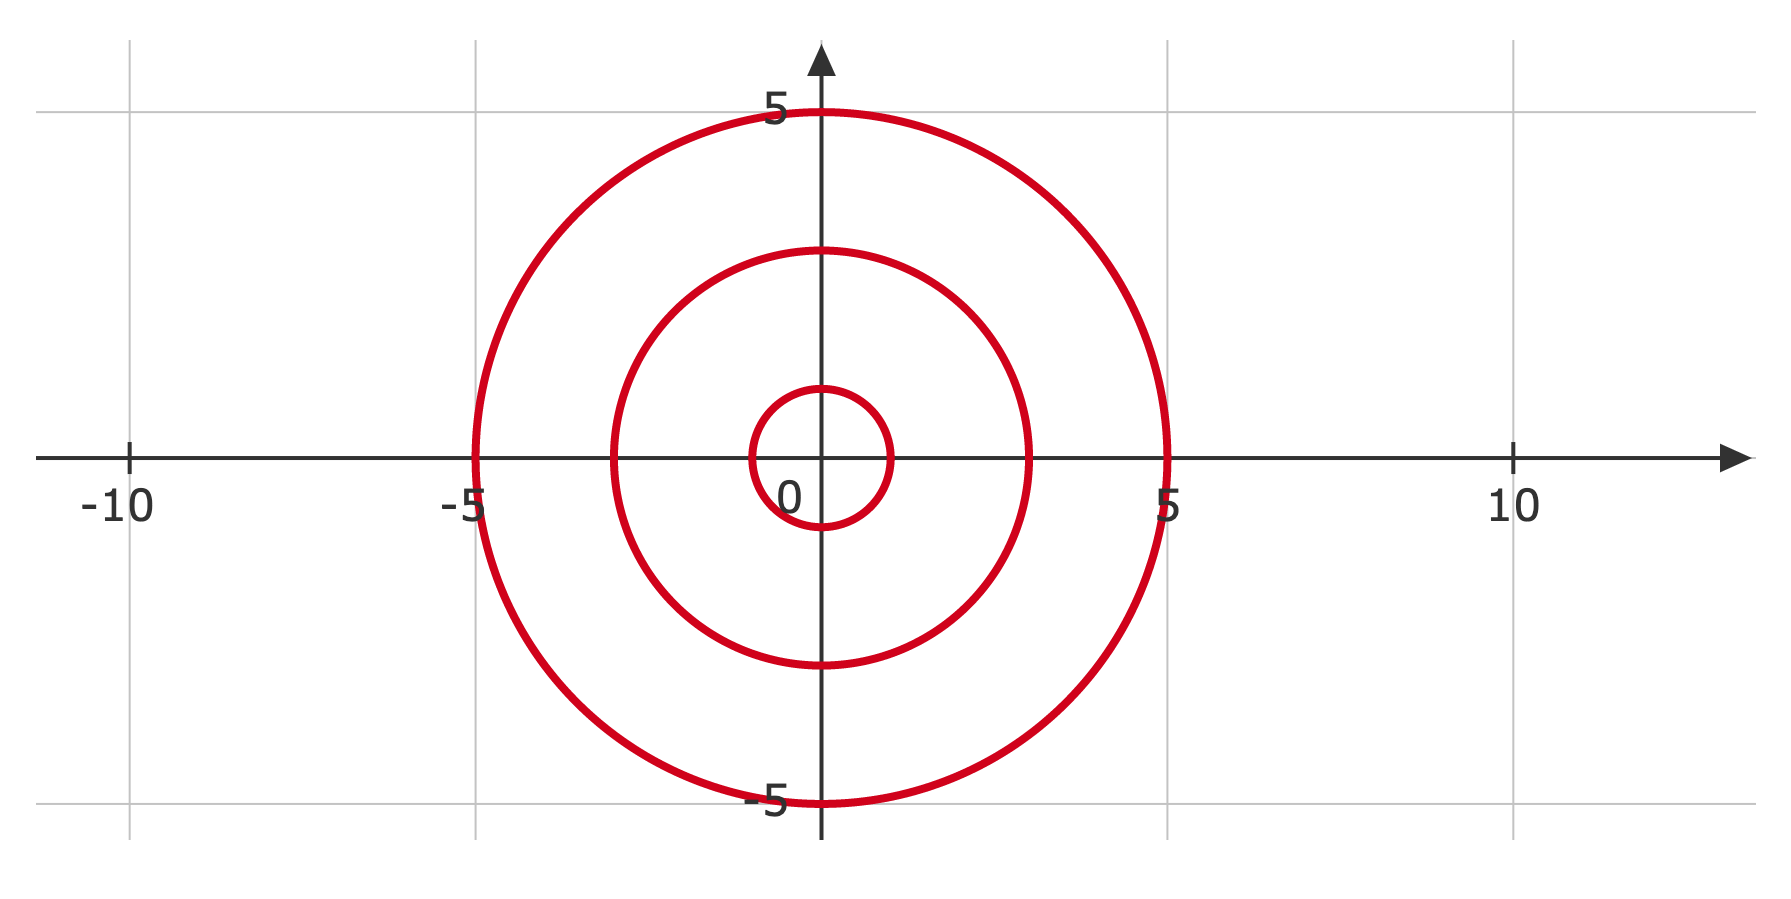
\includegraphics[width=0.7\linewidth]{figures/wk-6/fig-5.png}
	\end{center}
\end{ex}

\begin{marginfigure}
	\textbf{Exercise: } What are the flow lines of:
	\[\mathbf{V} = \frac{-y}{\sqrt{x^2+y^2}} \cdot \mathbf{i}+\frac{x}{\sqrt{x^2+y^2}} \cdot \mathbf{j}\]
\end{marginfigure}

\subsection{Divergence and Curl}
\begin{defn}[$\nabla$]
	The \textbf{del operator} in $n$-space is,
	\[\nabla=\left(\frac{\partial}{\partial x_1}, \frac{\partial}{\partial x_2}, \cdots, \frac{\partial}{\partial x_n}\right)\]
\end{defn}

\begin{marginfigure}
	The gradient of $f$ is obtained by taking the $\nabla$ operator and applying it to $f$.
\end{marginfigure}

\begin{defn}[$\operatorname{div} \mathbf{V}$]
	\sloppy The \textbf{divergence} of a vector field $\mathbf{V}$ on $\R^n$ is,
	\[\operatorname{div} \mathbf{V}= \nabla \cdot \mathbf{F} = \sum_{i=1}^n \frac{\partial V_i}{\partial x_i}=\frac{\partial V_1}{\partial x_1}+\cdots+\frac{\partial V_n}{\partial x_n}\]
\end{defn}

\begin{defn}[Solenoidal]
	If a vector field $\mathbf{V}$ on $\R^n$ has $\operatorname{div} \mathbf{V}(\mathbf{x}) = \mathbf{0}$, then $\mathbf{V}$ is called \textbf{solenoidal}.
\end{defn}

\begin{rmk}
	We evaluate the divergence at a point $\mathbf{x}$. 
	\begin{enumerate}
		\item If $\operatorname{div} \mathbf{V}(\mathbf{x}) < 0$, then $\mathbf{V}$ converges at $\mathbf{x}$
		\item If $\operatorname{div} \mathbf{V}(\mathbf{x}) > 0$, then $\mathbf{V}$ diverges at $\mathbf{x}$
	\end{enumerate}
\end{rmk}

\begin{defn}[$\operatorname{curl} \mathbf{V}$]
	The \textbf{curl} of a vector field $\mathbf{V}$ on $\R^3$ is,
	\[\operatorname{curl} \mathbf{V}=\nabla \times \mathbf{V}=\left|\begin{array}{ccc}
	\mathbf{i} & \mathbf{j} & \mathbf{k} \\
	\partial_x & \partial_y & \partial_z \\
	V_1 & V_2 & V_3
	\end{array}\right|\]
	which evaluates to,
	\[\left(\frac{\partial V_3}{\partial y}-\frac{\partial V_2}{\partial z}\right) \cdot \mathbf{i}+\left(\frac{\partial V_1}{\partial z}-\frac{\partial V_3}{\partial x}\right) \cdot \mathbf{j}+\left(\frac{\partial V_2}{\partial x}-\frac{\partial V_1}{\partial y}\right) \cdot \mathbf{k}\]
\end{defn}

\begin{marginfigure}
	$\operatorname{curl}(\mathbf{V})$ tells us how much the flow lines is $\mathbf{V}$ rotate. In particular, a gradient field has no center of rotation or else the level curves would intersect.
\end{marginfigure}

\begin{prop}[Curl of a Gradient]
	For any $C^2$ function $f$,
	\[\operatorname{curl} \nabla f = \nabla \times(\nabla f)=0\]
	That is, the curl of any gradient is the zero vector.
\end{prop}

\begin{cor}
	If $\operatorname{curl} \mathbf{V} = \nabla \times \mathbf{V} \neq 0$, then $\mathbf{V}$ is not a gradient field.
\end{cor}

\begin{prop}[Divergence of a Curl]
	For any $C^2$ vector field $\mathbf{V}$,
	\[\operatorname{div} \operatorname{curl} \mathbf{V}=\nabla \cdot(\nabla \times \mathbf{V})=0\]
	That is, the divergence of any curl is zero.
\end{prop}

\begin{cor}
	If $\operatorname{div} \mathbf{V} = \nabla \cdot \mathbf{V} \neq 0$, then $\mathbf{V}$ is not solenoidal.
\end{cor}